\documentclass[11pt]{article}
\usepackage[T1]{fontenc}
\usepackage[utf8]{inputenc}
\usepackage[portuguese]{babel}
\usepackage{amsmath}
\usepackage{graphicx}
\usepackage{float}
\usepackage{enumitem}

\graphicspath{{}}

\newcommand{\numpy}{{\tt numpy}}

\topmargin -.5in
\textheight 9in
\oddsidemargin -.25in
\evensidemargin -.25in
\textwidth 7in

\begin{document}

    \author{Lucas Emanuel Resck Domingues}
    \title{Aula prática 6
    \medbreak
    \large Imagens e SVD}
    \maketitle
    
    \medskip
    
    \begin{enumerate}
    
        \item %1
        
            No ambiente Scilab, para exibir as imagens \textit{img13\_Ema.png} e \textit{marinha.png}, foram executados os comandos \textit{imshow(imread("img13\_Ema.png"))} e \textit{imshow(imread("marinha.png"))}. A imagem é lida pelo Scilab e automaticamente é exibida na tela. Estes são os resultados:
        
            \begin{figure}[H]
                \centering                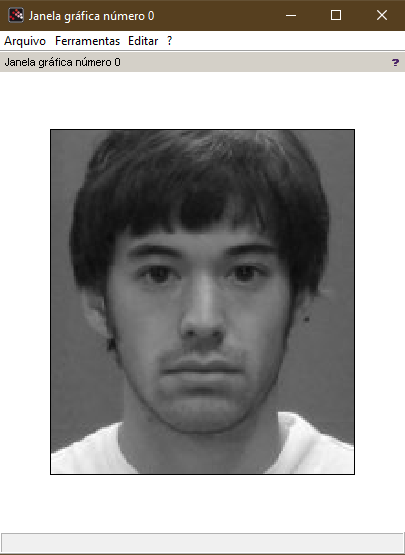
\includegraphics[scale=0.9]{1-1}
                \caption{Exibição da imagem \textit{img13\_Ema.png}.}
            \end{figure}
        
            \begin{figure}[H]
                \centering
                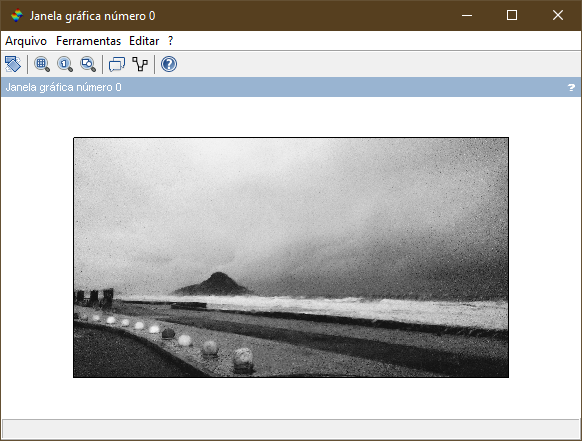
\includegraphics[]{1-2}
                \caption{Exibição da imagem \textit{marinha.png}.}
            \end{figure}
    
        \item %2
        
            A função \textit{compression} foi implementada em Scilab e está no arquivo \textit{Image compression function.sce}. Esta recebe uma matriz $A$ correspondente à imagem em preto e branco e um valor $p$ relativo à fração de valores singulares que vamos utilizar na compressão. Vamos testá-la para as imagens com alguns valores diferentes de $p$.
            
            A imagem \textit{img13\_Ema.png} original está à esquerda e a comprimida, à direita:
            
            \begin{figure}[H]
                \centering
                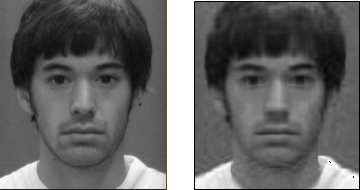
\includegraphics[]{2-1-10}
                \caption{Comparação para $p = 0,1$}
            \end{figure}
            
            \begin{figure}[H]
                \centering
                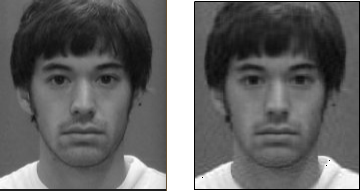
\includegraphics[]{2-1-15}
                \caption{Comparação para $p = 0,15$}
            \end{figure}
            
            \begin{figure}[H]
                \centering
                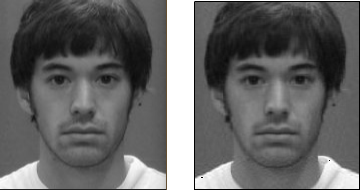
\includegraphics[]{2-1-20}
                \caption{Comparação para $p = 0,2$}
            \end{figure}
            
            \begin{figure}[H]
                \centering
                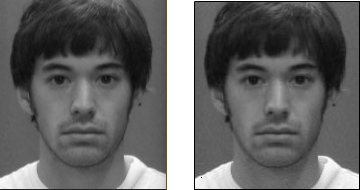
\includegraphics[]{2-1-25}
                \caption{Comparação para $p = 0,25$}
            \end{figure}
            
            Observe que, para essa imagem, $p = 0,25$ já é suficiente para que a imagem esteja relativamente boa, comparada à original. Não é instantâneo olhar para as duas imagens e apontar aquela original.
            
            Repetimos esse processo para a imagem \textit{marinha.png} (porém, agora, a original fica em cima e a comprimida, embaixo):
            
            \begin{figure}[H]
                \centering
                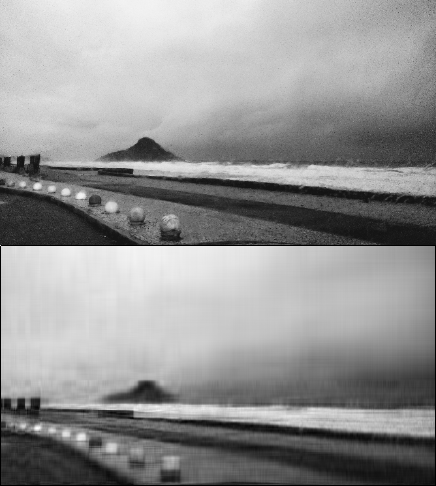
\includegraphics[]{2-2-005}
                \caption{Comparação para $p = 0,005$}
            \end{figure}
            
            \begin{figure}[H]
                \centering
                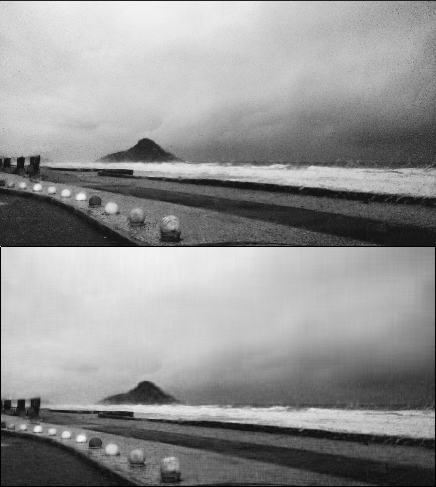
\includegraphics[]{2-2-015}
                \caption{Comparação para $p = 0,015$}
            \end{figure}
            
            \begin{figure}[H]
                \centering
                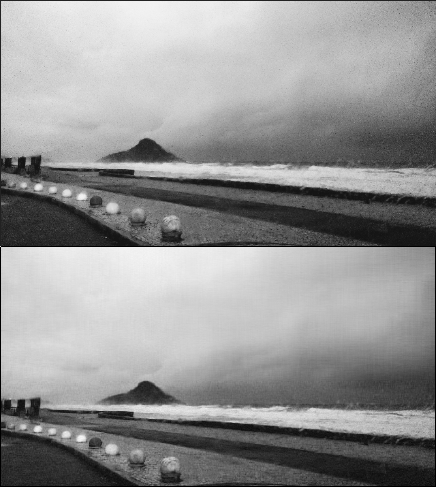
\includegraphics[]{2-2-025}
                \caption{Comparação para $p = 0,025$}
            \end{figure}
            
            \begin{figure}[H]
                \centering
                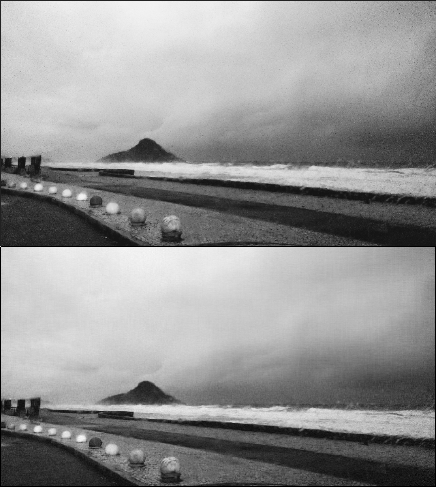
\includegraphics[]{2-2-035}
                \caption{Comparação para $p = 0,035$}
            \end{figure}
            
            Já para essa imagem, $p = 0,035$ é suficiente para que a imagem fique comparável à original.
        
    \end{enumerate}
\end{document}
\grid
\grid